\documentclass[11pt,a4paper,oneside]{book}

% Load custom Preamble (Packages, Styles, Colors, Listings, Callouts)
\usepackage[utf8]{inputenc}
\usepackage[T1]{fontenc}
\usepackage{lmodern}
\usepackage[margin=1in]{geometry}
\usepackage[table,dvipsnames]{xcolor}
\usepackage{graphicx}
\usepackage{listings}
\usepackage[most]{tcolorbox}
\usepackage{tikz}
\usetikzlibrary{shapes.geometric, arrows.meta, positioning, calc, shadows}
\usepackage{fancyhdr}
\usepackage{titlesec}
\usepackage{caption}
\usepackage{microtype}
\usepackage{parskip}
\usepackage{amsmath,amssymb}
\usepackage{hyperref}

% --- Custom Colors ---
\definecolor{pyblue}{HTML}{1E40AF}      % Deep Python Blue
\definecolor{pyyellow}{HTML}{D97706}    % Warm Python Amber
\definecolor{pygreen}{HTML}{059669}     % Energetic Green
\definecolor{pypurple}{HTML}{7C3AED}    % Wizard Purple
\definecolor{codegray}{HTML}{4B5563}    % Code comment gray
\definecolor{codebg}{HTML}{F8FAFC}      % Code background light gray
\definecolor{codeframe}{HTML}{CBD5E1}   % Code box border
\definecolor{snackbg}{HTML}{EFF6FF}     % Pro tip background
\definecolor{snackborder}{HTML}{3B82F6} % Pro tip border
\definecolor{pitfallbg}{HTML}{FEF2F2}   % Alert background
\definecolor{pitfallborder}{HTML}{EF4444}% Alert border
\definecolor{chucklebg}{HTML}{FFFBEB}   % Funny break background
\definecolor{chuckleborder}{HTML}{F59E0B}% Funny break border
\definecolor{labbg}{HTML}{ECFDF5}       % Lab challenge background
\definecolor{labborder}{HTML}{10B981}   % Lab challenge border

% --- Hyperref Setup ---
\hypersetup{
    colorlinks=true,
    linkcolor=pypurple,
    citecolor=pygreen,
    urlcolor=pyblue,
    pdftitle={Snake Bytes: Python Programming Fundamentals},
    pdfauthor={The Antigravity Python Wizard}
}

% --- Page Style & Headers ---
\pagestyle{fancy}
\fancyhf{}
\fancyhead[L]{\small\color{codegray}\leftmark}
\fancyhead[R]{\small\color{pypurple}\bfseries Snake Bytes: Python Fundamentals}
\fancyfoot[C]{\small\color{codegray}\thepage}
\renewcommand{\headrulewidth}{0.4pt}
\renewcommand{\footrulewidth}{0pt}

% --- Section & Chapter Heading Formatting ---
\titleformat{\chapter}[display]
  {\normalfont\huge\bfseries\color{pypurple}}
  {\Large\color{pyyellow}\chaptertitlename\ \thechapter}
  {10pt}
  {\Huge}

\titleformat{\section}
  {\normalfont\Large\bfseries\color{pyblue}}
  {\thesection}{1em}{}

\titleformat{\subsection}
  {\normalfont\large\bfseries\color{pygreen}}
  {\thesubsection}{1em}{}

% --- Listings (Code Syntax Highlighting) Setup ---
\lstset{
    language=Python,
    backgroundcolor=\color{codebg},
    basicstyle=\ttfamily\small\color{black},
    keywordstyle=\bfseries\color{pypurple},
    stringstyle=\color{pygreen},
    commentstyle=\itshape\color{codegray},
    numberstyle=\tiny\color{codegray},
    numbers=left,
    numbersep=10pt,
    stepnumber=1,
    showstringspaces=false,
    tabsize=4,
    breaklines=true,
    breakatwhitespace=true,
    frame=none,
    captionpos=b,
    keepspaces=true
}

% Styled Code Box Container
\newtcblisting{pycode}[2][]{
    toptitle=2mm,
    bottomtitle=2mm,
    colback=codebg,
    colframe=codeframe,
    coltitle=black,
    fonttitle=\bfseries\ttfamily\small,
    title={\small\hspace{1mm} Python Listing: #2},
    enhanced,
    attach boxed title to top left={yshift=-2mm,xshift=3mm},
    boxed title style={colback=codeframe!30!white,colframe=codeframe,arc=2mm},
    arc=3mm,
    drop shadow=black!10!white,
    listing only,
    listing options={
        language=Python,
        basicstyle=\ttfamily\small,
        keywordstyle=\bfseries\color{pypurple},
        stringstyle=\color{pygreen},
        commentstyle=\itshape\color{codegray},
        numberstyle=\tiny\color{codegray},
        numbers=left,
        numbersep=8pt,
        breaklines=true,
        showstringspaces=false
    },
    #1
}

% --- Custom Callout Boxes ---
% 1. Snake Snack (Pro Tip)
\newtcolorbox{snakesnack}[1]{
    enhanced,
    colback=snackbg,
    colframe=snackborder,
    arc=3mm,
    fonttitle=\bfseries\color{snackborder},
    title={ Snake Snack (Pro Tip): #1},
    drop shadow=snackborder!20!white
}

% 2. Viper Pitfall (Common Error)
\newtcolorbox{viperpitfall}[1]{
    enhanced,
    colback=pitfallbg,
    colframe=pitfallborder,
    arc=3mm,
    fonttitle=\bfseries\color{pitfallborder},
    title={ Viper Pitfall (Watch Out!): #1},
    drop shadow=pitfallborder!20!white
}

% 3. Chuckle Break (Humor & Analogy)
\newtcolorbox{chucklebreak}[1]{
    enhanced,
    colback=chucklebg,
    colframe=chuckleborder,
    arc=3mm,
    fonttitle=\bfseries\color{chuckleborder},
    title={ Chuckle Break: #1},
    drop shadow=chuckleborder!20!white
}

% 4. Snake Lab (Interactive Exercise)
\newtcolorbox{snakelab}[1]{
    enhanced,
    colback=labbg,
    colframe=labborder,
    arc=3mm,
    fonttitle=\bfseries\color{labborder},
    title={ Snake Lab Challenge: #1},
    drop shadow=labborder!20!white
}


\begin{document}

% --- Front Matter ---
\frontmatter
\begin{titlepage}
\centering
\vspace*{1cm}

{\Huge \bfseries \color{pypurple} SNAKE BYTES \par}
\vspace{0.4cm}
{\Large \bfseries \color{pyyellow} A Whimsical \& Funny Guide to Python Programming Fundamentals \par}

\vspace{0.8cm}
\rule{\linewidth}{1.5pt}
\vspace{0.8cm}

\begin{figure}[h!]
    \centering
    
\includegraphics[width=0.65\textwidth]{images/cover_art.jpg}
\end{figure}

\vfill

{\Large \textbf{By Sudheer K. Mohammed} \par}
\vspace{0.3cm}
{\small Illustrated by AI Artificers $\cdot$ Code Verified by Literal Computers \par}
\vspace{0.5cm}
{\small \color{codegray} First Edition --- 2026 \par}

\end{titlepage}


\clearpage
\tableofcontents
\clearpage

% --- Main Matter ---
\mainmatter

\chapter{Welcome to the Pit: Variables \& Data Types}

\begin{figure}[h!]
    \centering
    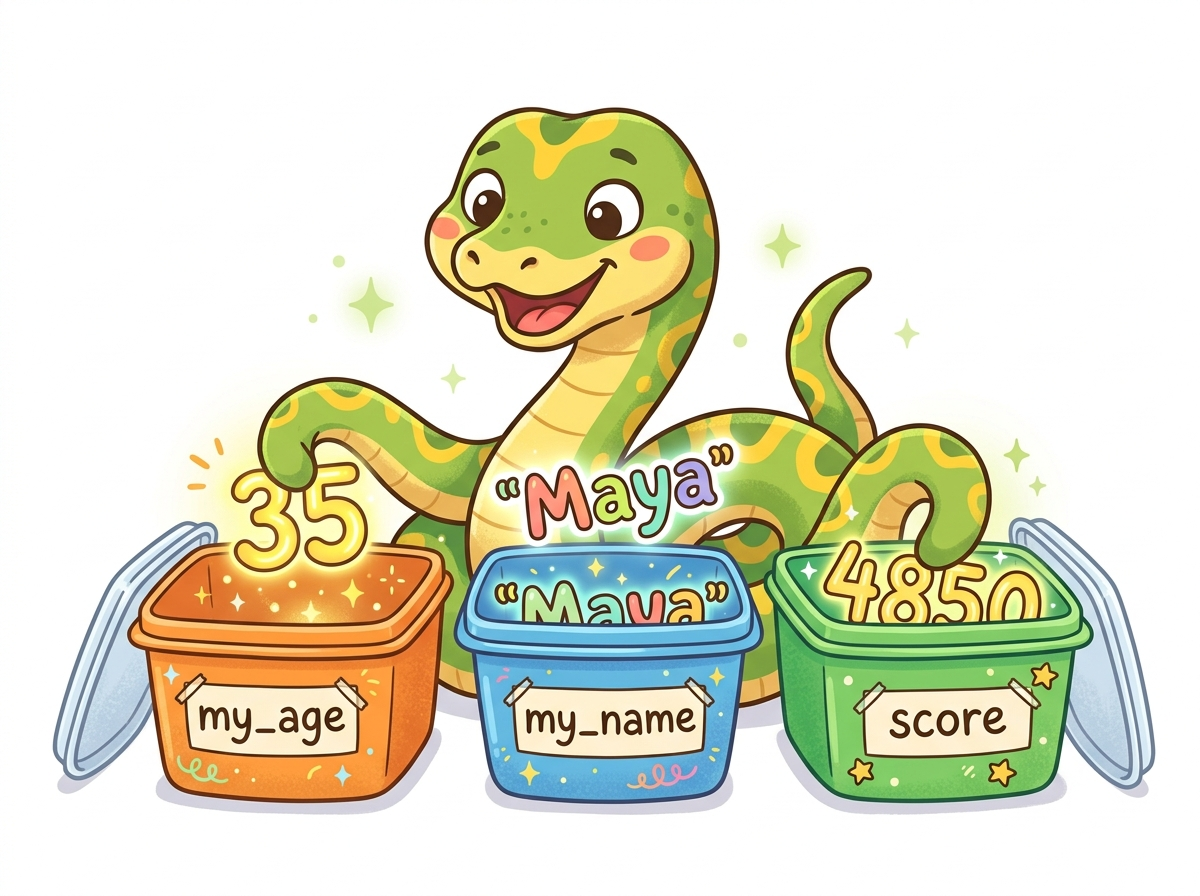
\includegraphics[width=0.75\textwidth]{images/ch1_tupperware.jpg}
    \caption{Variables in Python are like labeled Tupperware containers holding your valuable data.}
\end{figure}

\section{What is Code Anyway?}

Welcome, courageous snake charmer! Programming is simply the art of giving orders to a very fast, extremely loyal, but shockingly literal silicon rock called a CPU. If you tell a CPU to jump off a bridge, it won't ask ``Why?''; it will ask ``At what speed and angle in meters per second?''.

Python is one of the most friendly programming languages ever invented. Instead of cryptic binary numbers or terrifying C code with pointer arrows, Python reads almost like plain English with strict punctuation habits.

\section{Variables: Labeled Tupperware Containers}

Imagine your computer's Memory (RAM) as a giant kitchen filled with blank plastic Tupperware containers. A \textbf{variable} is just a friendly sticky note label you slap onto one of those containers so you can find your data later.

In Python, creating a variable is as simple as using the equals sign (\texttt{=}), which is called the \textbf{assignment operator}.

\begin{pycode}{Variables in Action}
# Slapping sticky notes on memory containers
my_age = 25
my_name = "Maya the Python"
is_hungry = True
coffee_cups = 3.5

# Displaying our loot to the world
print(my_name)
print("Coffee cups consumed today:", coffee_cups)
\end{pycode}

\begin{chucklebreak}{Why not store everything in your brain?}
Because human brains forget where they parked their car 10 minutes ago, whereas computer memory can store millions of numbers with 100\% precision until you pull the plug!
\end{chucklebreak}

\section{The Four Fundamental Data Types}

Python automatically figures out what kind of data you put inside your container. Here are the big four fundamental types:

\begin{enumerate}
    \item \textbf{Integer (\texttt{int}):} Whole numbers without decimals. E.g., \texttt{42}, \texttt{-7}, \texttt{1000}.
    \item \textbf{Float (\texttt{float}):} Floating-point decimal numbers. E.g., \texttt{3.14159}, \texttt{-0.001}.
    \item \textbf{String (\texttt{str}):} Text characters enclosed in quotes. E.g., \texttt{"Hello World!"}, \texttt{'Snakes rule'}.
    \item \textbf{Boolean (\texttt{bool}):} Absolute truth values. Only two exist: \texttt{True} or \texttt{False}.
\end{enumerate}

\begin{pycode}{Checking Data Types with type()}
x = 100
y = 3.14
z = "Python"
flag = True

print(type(x))     # <class 'int'>
print(type(y))     # <class 'float'>
print(type(z))     # <class 'str'>
print(type(flag))  # <class 'bool'>
\end{pycode}

\begin{viperpitfall}{Quotations Matter!}
Mixing up strings and numbers is a classic rookie mistake!
\texttt{x = 5} is a number you can do math with.
\texttt{x = "5"} is a piece of text! If you add \texttt{"5" + "5"}, Python won't give you \texttt{10} --- it will give you \texttt{"55"}!
\end{viperpitfall}

\section{Dynamic f-strings: Talking to Humans}

When you want to blend variables seamlessly into sentences, Python's \textbf{f-strings} (formatted string literals) are your best friend. Put an \texttt{f} right before the opening quote, and put variable names inside curly braces \texttt{\{\}}.

\begin{pycode}{f-String Magic}
name = "Cornelius"
pet = "Python"
age = 4

# Elegant f-string output
greeting = f"Hello, I am {name} the {pet}, and I am {age} years old!"
print(greeting)
\end{pycode}

\section{Code Example: The Wizard's Shopping Receipt}

Let's look at a practical example combining string input, type conversion, basic math, and f-strings to calculate a total potion bill.

\begin{pycode}{Shopping Receipt Calculator}
item_name = "Dragon Health Potion"
item_price = 15.50
quantity = 3
tax_rate = 0.08  # 8% tax

# Math calculations
subtotal = item_price * quantity
tax_amount = subtotal * tax_rate
grand_total = subtotal + tax_amount

# Printable receipt
print("--- WIZARD INN RECEIPT ---")
print(f"Item: {item_name} (x{quantity})")
print(f"Subtotal: ${subtotal:.2f}")
print(f"Tax (8%): ${tax_amount:.2f}")
print(f"Grand Total: ${grand_total:.2f}")
print("--------------------------")
\end{pycode}

\begin{snakesnack}{Variable Naming Rules}
Variable names in Python should be lowercase with words separated by underscores (called \texttt{snake\_case}). 
\begin{itemize}
    \item Good: \texttt{dragon\_health}, \texttt{user\_score\_2}
    \item Bad: \texttt{2nd\_user} (cannot start with a number!)
    \item Dangerous: \texttt{class}, \texttt{def}, \texttt{if} (these are reserved keywords!)
\end{itemize}
\end{snakesnack}

\section{Practice Problems \& Exercises}

Try solving these 3 practice problems to test your knowledge of variables and data types!

\begin{snakelab}{Problem 1.1: The Dragon's Loot Splitter (Easy)}
Write a script that divides $100$ gold coins equally among $3$ adventurer party members. 
\begin{itemize}
    \item Calculate how many coins each member gets using integer division (\texttt{//}).
    \item Calculate how many coins are left over for the dragon using the modulo operator (\texttt{\%}).
    \item Print the results using f-strings!
\end{itemize}
\end{snakelab}

\begin{pycode}{Solution 1.1: Dragon's Loot Splitter}
total_gold = 100
party_members = 3

coins_per_person = total_gold // party_members  # 33
leftover_gold = total_gold % party_members       # 1

print(f"Each adventurer receives {coins_per_person} gold coins.")
print(f"The greedy dragon keeps {leftover_gold} coin as tribute!")
\end{pycode}

\begin{snakelab}{Problem 1.2: Temperature Converter (Medium)}
Write a script that converts a temperature from Fahrenheit to Celsius using the formula:
\[ C = (F - 32) \times \frac{5}{9} \]
Test your program with $F = 98.6$ degrees and format the Celsius result to 1 decimal place.
\end{snakelab}

\begin{pycode}{Solution 1.2: Temperature Converter}
temp_f = 98.6
temp_c = (temp_f - 32) * (5 / 9)

print(f"{temp_f} degrees Fahrenheit is equal to {temp_c:.1f} degrees Celsius.")
\end{pycode}

\begin{snakelab}{Problem 1.3: Funny RPG Character Generator (Spicy)}
Write a script that stores a hero name, a weapon name, an agility level, and a luck score. 
Print out a comical character stats sheet with formatted lines and string repeating (e.g. \texttt{"=" * 30}).
\end{snakelab}

\begin{pycode}{Solution 1.3: RPG Character Generator}
hero_name = "Sir Reginald the Fluffy"
weapon = "Spoon of Doom"
agility = 12
luck = 99.5

banner = "=" * 32
print(banner)
print(f" HERO STATS: {hero_name.upper()}")
print(banner)
print(f" * Primary Weapon : {weapon}")
print(f" * Agility Score  : {agility}")
print(f" * Luck Rating    : {luck:.1f}%")
print(banner)
\end{pycode}

\chapter{The Forking Path: Control Flow \& Logic}

\begin{figure}[h!]
    \centering
    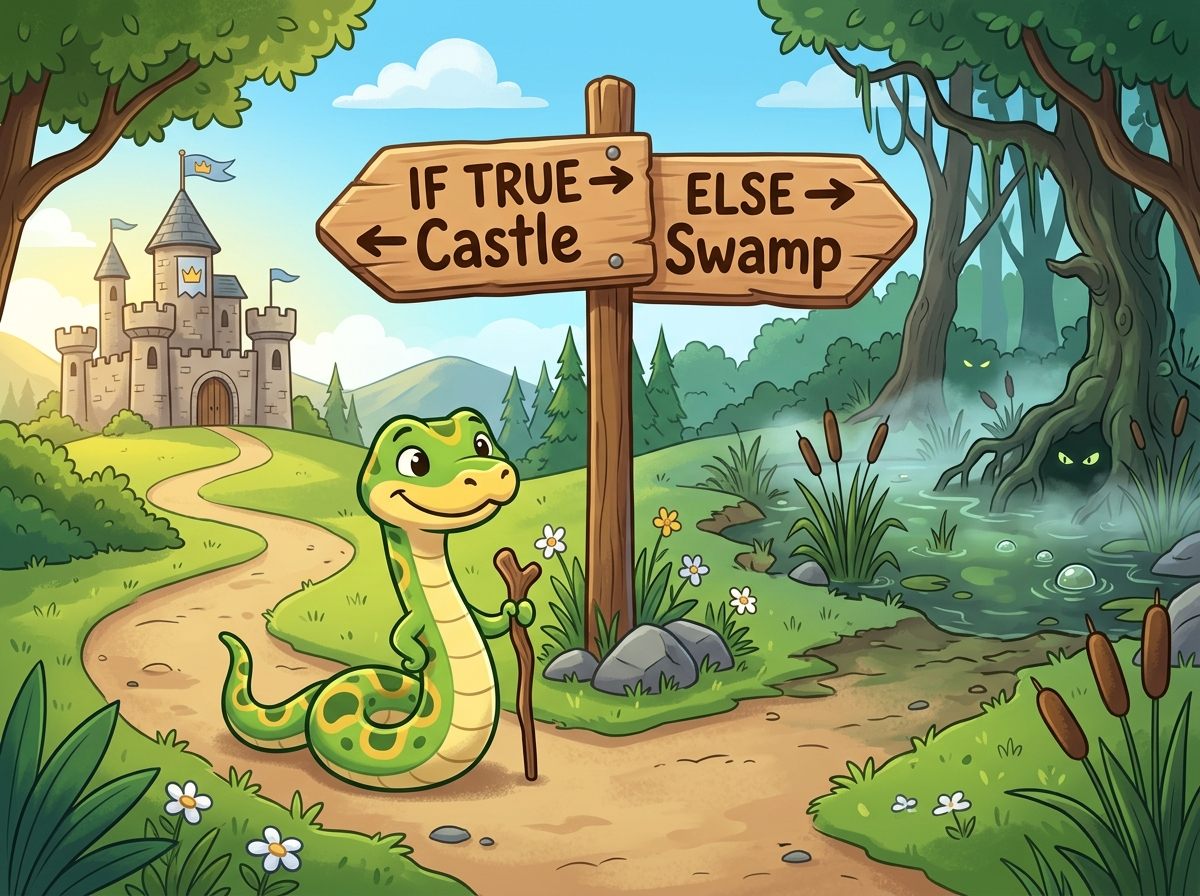
\includegraphics[width=0.75\textwidth]{images/ch2_crossroads.jpg}
    \caption{Control flow lets your code make choices like choosing a path at a crossroad.}
\end{figure}

\section{Life is Full of Choices... and So is Code!}

Without decisions, a program would just run top-to-bottom like a train on a single track. But real life requires choices: \textit{If} it rains, take an umbrella; \textit{else}, wear sunglasses!

In Python, we direct the flow of execution using \textbf{conditional statements}: \texttt{if}, \texttt{elif} (short for else-if), and \texttt{else}.

\section{The Honest Truth: Booleans \& Comparison Operators}

Before making decisions, Python evaluates questions to find if they are \texttt{True} or \texttt{False}. We ask questions using comparison operators:

\begin{table}[h!]
\centering
\begin{tabular}{|c|l|c|}
\hline
\rowcolor{pyblue!20} \textbf{Operator} & \textbf{Meaning} & \textbf{Example ($5$ vs $10$)} \\ \hline
\texttt{==} & Equals (Are they identical?) & \texttt{5 == 10} $\rightarrow$ \texttt{False} \\ \hline
\texttt{!=} & Not Equals (Are they different?) & \texttt{5 != 10} $\rightarrow$ \texttt{True} \\ \hline
\texttt{>} & Greater Than & \texttt{5 > 10} $\rightarrow$ \texttt{False} \\ \hline
\texttt{<} & Less Than & \texttt{5 < 10} $\rightarrow$ \texttt{True} \\ \hline
\texttt{>=} & Greater Than or Equal To & \texttt{5 >= 5} $\rightarrow$ \texttt{True} \\ \hline
\texttt{<=} & Less Than or Equal To & \texttt{10 <= 5} $\rightarrow$ \texttt{False} \\ \hline
\end{tabular}
\caption{Python Comparison Operators}
\end{table}

\begin{viperpitfall}{The Single vs Double Equals Trap!}
Single equals (\texttt{=}) is for \textbf{assignment} (putting stuff in a container).
Double equals (\texttt{==}) is for \textbf{comparison} (asking if two things match).
If you write \texttt{if age = 18:}, Python will throw a syntax error and scold you!
\end{viperpitfall}

\section{The Choose-Your-Own-Adventure Branch}

Here is how you write a basic conditional block in Python:

\begin{pycode}{If-Elif-Else in Action}
dragon_hunger_level = 85

if dragon_hunger_level > 90:
    print("RUN FOR YOUR LIFE! The dragon wants to eat you!")
elif dragon_hunger_level > 50:
    print("Toss a marshmallow to buy yourself 10 seconds.")
else:
    print("The dragon is sleeping peacefully. You may pass.")
\end{pycode}

\section{Logical Operators: Combining Questions}

Sometimes you need to check multiple conditions at once:
\begin{itemize}
    \item \textbf{\texttt{and}:} Returns \texttt{True} ONLY if BOTH conditions are True.
    \item \textbf{\texttt{or}:} Returns \texttt{True} if AT LEAST ONE condition is True.
    \item \textbf{\texttt{not}:} Flips the boolean value (\texttt{True} becomes \texttt{False}).
\end{itemize}

\begin{pycode}{Combining Logic}
has_key = True
knows_password = False
is_admin = True

# Door opening logic
if (has_key and knows_password) or is_admin:
    print("ACCESS GRANTED! Welcome to the secret lair.")
else:
    print("ACCESS DENIED! The alarm is ringing!")
\end{pycode}

\section{Code Example: Theme Park Ticket Tier Classifier}

Let's examine how real-world nested conditions classify theme park admission ticket prices based on visitor age and height requirements.

\begin{pycode}{Theme Park Ticket Pricing}
visitor_age = 14
height_cm = 155
is_weekend = True

# Base pricing tiers
if visitor_age < 5:
    ticket_price = 0.00
    category = "Toddler (Free)"
elif visitor_age <= 17:
    ticket_price = 15.00
    category = "Youth"
else:
    ticket_price = 25.00
    category = "Adult"

# Weekend surcharge
if is_weekend and ticket_price > 0:
    ticket_price += 5.00

# Height check for rollercoaster
can_ride_rollercoaster = height_cm >= 140

print(f"Ticket Category: {category}")
print(f"Final Ticket Price: ${ticket_price:.2f}")
print(f"Rollercoaster Eligible: {can_ride_rollercoaster}")
\end{pycode}

\begin{snakesnack}{Indentation Rule}
Always use 4 spaces per indentation level. Do not mix tabs and spaces in the same file unless you want to trigger Python's infamous \texttt{IndentationError}!
\end{snakesnack}

\section{Practice Problems \& Exercises}

Put your decision-making skills to the test with these 3 logic exercises!

\begin{snakelab}{Problem 2.1: The Magic Bouncer (Easy)}
Write a program with variables \texttt{age = 19} and \texttt{is\_vip = False}.
\begin{itemize}
    \item If age is 21 or older, OR if \texttt{is\_vip} is True, print ``Welcome to the Python Lounge!''
    \item Otherwise, print ``Entry denied! Come back when you're older.''
\end{itemize}
\end{snakelab}

\begin{pycode}{Solution 2.1: Magic Bouncer}
age = 19
is_vip = False

if age >= 21 or is_vip:
    print("Welcome to the Python Lounge!")
else:
    print("Entry denied! Come back when you're older.")
\end{pycode}

\begin{snakelab}{Problem 2.2: Leap Year Detector (Medium)}
A year is a leap year if it is divisible by $4$, EXCEPT if it is divisible by $100$, UNLESS it is also divisible by $400$.
Write a script testing \texttt{year = 2024} and \texttt{year = 1900} to print whether each year is a leap year!
\end{snakelab}

\begin{pycode}{Solution 2.2: Leap Year Detector}
year = 2024

if (year % 4 == 0 and year % 100 != 0) or (year % 400 == 0):
    print(f"Year {year} is a LEAP YEAR!")
else:
    print(f"Year {year} is a standard year.")
\end{pycode}

\begin{snakelab}{Problem 2.3: RPG Critical Hit Calculator (Spicy)}
Given a player's attack power of $50$ and a random dice roll value between $1$ and $20$:
\begin{itemize}
    \item If dice roll is $20$: Critical hit! Multiply damage by $3$.
    \item If dice roll is $15$ to $19$: Strong hit! Multiply damage by $1.5$.
    \item If dice roll is $2$ to $14$: Normal hit! Deal base damage ($50$).
    \item If dice roll is $1$: Critical fumble! Deal $0$ damage and print a clumsy message.
\end{itemize}
\end{snakelab}

\begin{pycode}{Solution 2.3: Critical Hit Calculator}
base_attack = 50
dice_roll = 20  # Simulated roll

if dice_roll == 20:
    damage = base_attack * 3
    print(f"NAT 20! CRITICAL HIT! Dealt {damage} damage!")
elif dice_roll >= 15:
    damage = base_attack * 1.5
    print(f"Great hit! Dealt {damage:.0f} damage.")
elif dice_roll >= 2:
    damage = base_attack
    print(f"Normal hit. Dealt {damage} damage.")
else:
    damage = 0
    print("CRITICAL FUMBLE! You tripped over your own cape and dealt 0 damage!")
\end{pycode}

\chapter{Round and Round We Go: Loops}

\begin{figure}[h!]
    \centering
    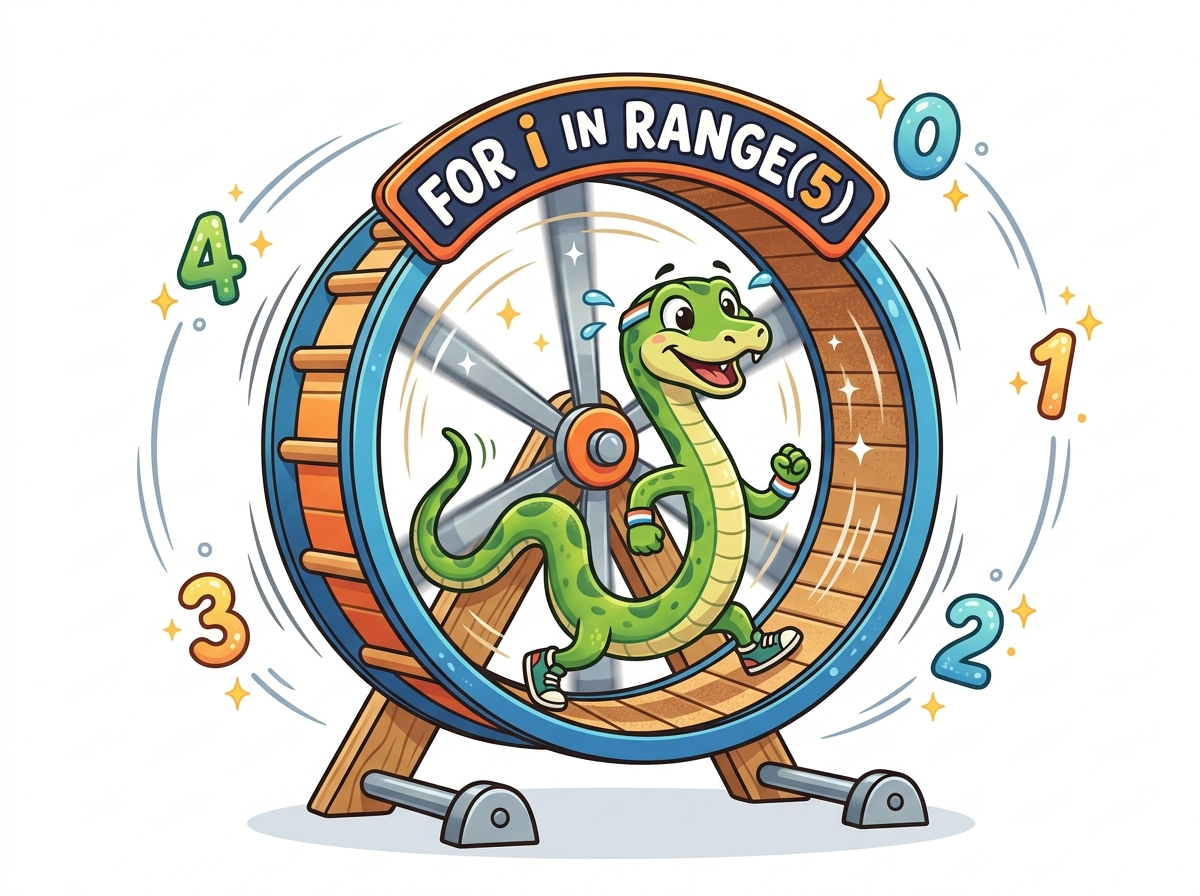
\includegraphics[width=0.75\textwidth]{images/ch3_hamster_wheel.jpg}
    \caption{Loops let your code repeat tasks like running on a hamster wheel without getting tired!}
\end{figure}

\section{Why Do Computers Love Repetition?}

If you ask a human to say ``I will not code in assembly'' 1,000 times, they will cry by iteration 14. If you ask Python to do it, it completes the task in 0.0002 seconds and asks for more!

In Python, we have two primary types of loops:
\begin{enumerate}
    \item \textbf{\texttt{for} loops:} Repeat a fixed number of times or iterate over items in a collection.
    \item \textbf{\texttt{while} loops:} Keep repeating as long as a condition stays \texttt{True}.
\end{enumerate}

\section{The Counting Wizard: \texttt{for} Loops \& \texttt{range()}}

The \texttt{range()} function is Python's number generator spell.

\begin{pycode}{Counting with range()}
# Count from 0 up to (but NOT including) 5
for i in range(5):
    print(f"Hamster wheel spin #{i}")

# range(start, stop, step)
print("Countdown:")
for count in range(10, 0, -2):
    print(f"{count}...")
print("BLAST OFF!")
\end{pycode}

\begin{chucklebreak}{Zero-Based Indexing}
Why does \texttt{range(5)} give us \texttt{0, 1, 2, 3, 4}? Because programmers start counting at zero! Why? Because in early memory architectures, index zero meant ``zero offsets from the beginning of the memory array''. Also, it keeps computer scientists feeling special.
\end{chucklebreak}

\section{The Relentless \texttt{while} Loop}

A \texttt{while} loop checks a boolean condition before every lap. If the condition is \texttt{True}, it executes the loop body. If it turns \texttt{False}, it stops.

\begin{pycode}{The Energy Counter}
energy = 3

while energy > 0:
    print(f"Coding... Energy left: {energy}")
    energy -= 1  # Equivalent to energy = energy - 1

print("Out of energy! Time for coffee!")
\end{pycode}

\begin{viperpitfall}{The Infinite Loop of Doom!}
If you forget to update your counter or condition inside a \texttt{while} loop:
\begin{lstlisting}[language=Python]
# DANGER: THIS WILL RUN FOREVER!
while True:
    print("I forgot to add an exit condition!")
\end{lstlisting}
If your terminal starts spinning out of control, press \texttt{CTRL + C} to break free!
\end{viperpitfall}

\section{Escape Hatches: \texttt{break} and \texttt{continue}}

- \textbf{\texttt{break}:} Instantly aborts the loop and jumps outside.
- \textbf{\texttt{continue}:} Skips the rest of the current lap and jumps straight to the next lap!

\begin{pycode}{Using break and continue}
for num in range(1, 10):
    if num == 3:
        print("Skipping 3 because it's unlucky!")
        continue
    if num == 7:
        print("Hit 7! Jackpot! Stopping loop.")
        break
    print(f"Processing item {num}")
\end{pycode}

\section{Code Example: Nested Loops Grid Generator}

Loops inside loops allow us to construct multi-dimensional grids, such as multiplication tables.

\begin{pycode}{Nested Loop Multiplication Table}
# Print a 4x4 multiplication table grid
print("--- 4x4 MULTIPLICATION TABLE ---")
for row in range(1, 5):
    row_text = ""
    for col in range(1, 5):
        product = row * col
        row_text += f"{product:4d}"  # Width of 4 spaces
    print(row_text)
\end{pycode}

\section{Practice Problems \& Exercises}

Loop around these 3 practice challenges!

\begin{snakelab}{Problem 3.1: The Classic FizzBuzz (Easy)}
Write a \texttt{for} loop that counts from $1$ to $20$.
\begin{itemize}
    \item If the number is divisible by $3$, print \texttt{"Fizz"}.
    \item If the number is divisible by $5$, print \texttt{"Buzz"}.
    \item If divisible by BOTH $3$ and $5$, print \texttt{"FizzBuzz"}.
    \item Otherwise, print the number itself!
\end{itemize}
\end{snakelab}

\begin{pycode}{Solution 3.1: FizzBuzz}
for n in range(1, 21):
    if n % 3 == 0 and n % 5 == 0:
        print("FizzBuzz")
    elif n % 3 == 0:
        print("Fizz")
    elif n % 5 == 0:
        print("Buzz")
    else:
        print(n)
\end{pycode}

\begin{snakelab}{Problem 3.2: Bank Vault PIN Retries (Medium)}
Write a \texttt{while} loop that simulates a bank vault security system with a max limit of $3$ attempts.
Simulate guesses starting with \texttt{1111}, \texttt{2222}, and ending with correct PIN \texttt{7777}.
Print access status for each attempt and abort early if correct!
\end{snakelab}

\begin{pycode}{Solution 3.2: Bank Vault Security}
correct_pin = "7777"
guesses = ["1111", "2222", "7777"]
attempt = 0
max_attempts = 3

while attempt < max_attempts:
    current_guess = guesses[attempt]
    attempt += 1
    print(f"Attempt {attempt}/{max_attempts}: Testing PIN '{current_guess}'...")
    
    if current_guess == correct_pin:
        print("SUCCESS! Vault opened!")
        break
    else:
        print("WRONG PIN!")
else:
    print("LOCKDOWN! Max attempts exceeded.")
\end{pycode}

\begin{snakelab}{Problem 3.3: Star Pyramid Pattern (Spicy)}
Write nested \texttt{for} loops to print an ascending pyramid of stars (\texttt{*}) with $5$ rows.
Row 1 has 1 star, Row 2 has 2 stars, ..., Row 5 has 5 stars.
\end{snakelab}

\begin{pycode}{Solution 3.3: Star Pyramid Pattern}
total_rows = 5

for row in range(1, total_rows + 1):
    stars = "*" * row
    print(stars)
\end{pycode}

\chapter{Reusable Spellbooks: Functions}

\begin{figure}[h!]
    \centering
    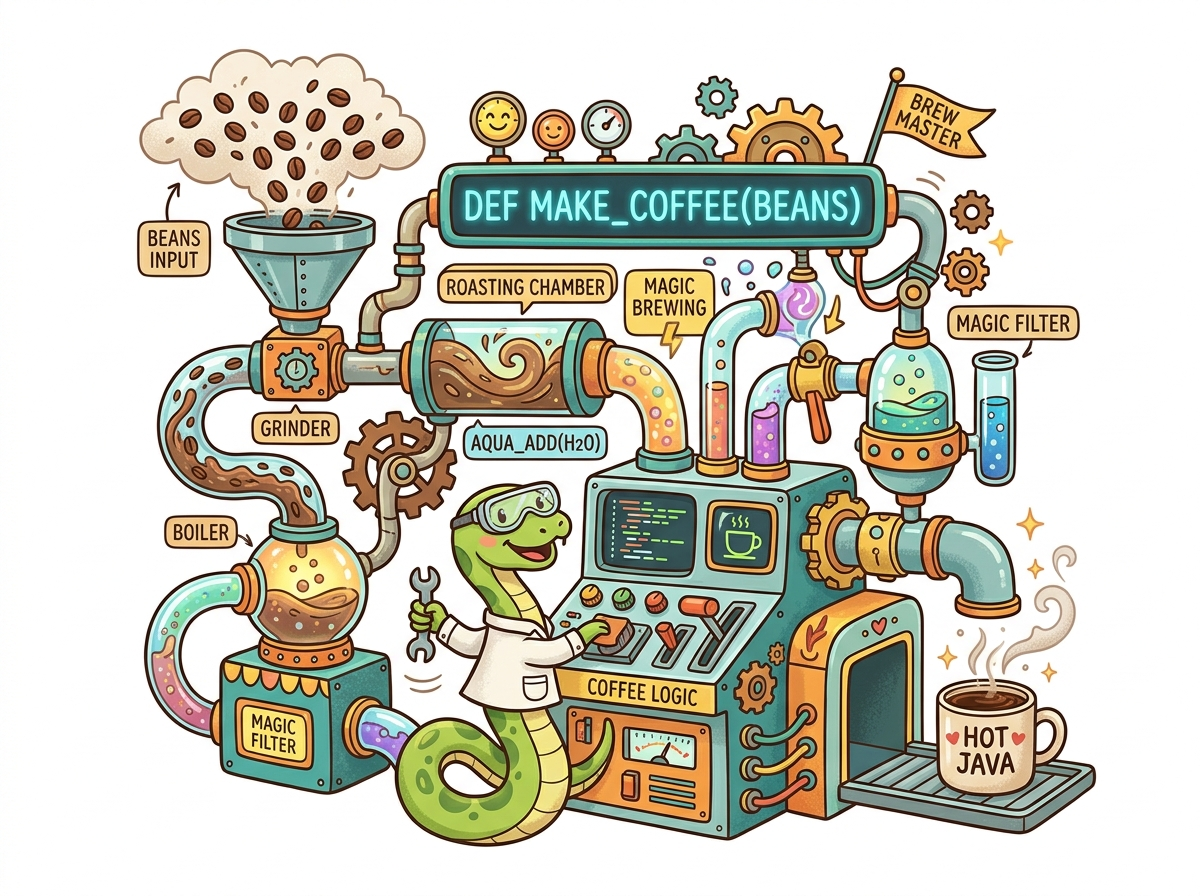
\includegraphics[width=0.75\textwidth]{images/ch4_magic_machine.jpg}
    \caption{Functions are like magic coffee brewing machines: feed them inputs, get delicious results!}
\end{figure}

\section{Don't Repeat Yourself (DRY Principle)}

Copying and pasting the same code 5 times in your program is a crime against humanity. If you find a bug in that code later, you will have to fix it in 5 different places (and you will forget place \#4).

A \textbf{function} is a bundled block of reusable code. You define it once, name it, and call it whenever you need it!

\section{Defining and Calling Functions}

We use the keyword \texttt{def} to define a function, followed by the function name and parentheses \texttt{()}.

\begin{pycode}{Basic Function}
# 1. Defining the magic spell
def cast_fireball():
    print("WHOOSH! A fiery explosion illuminates the room!")

# 2. Calling the spell
cast_fireball()
cast_fireball()
\end{pycode}

\section{Parameters \& Arguments: Feeding the Machine}

Functions become 10x more useful when you feed them input values called \textbf{parameters}.

\begin{pycode}{Functions with Inputs}
def greet_wizard(wizard_name, spell_element="Ice"):
    print(f"Greetings, Archmage {wizard_name}! Master of {spell_element}!")

# Positional arguments
greet_wizard("Gandalf", "Light")

# Using default parameter values
greet_wizard("Merlin")
\end{pycode}

\section{Return Values: Receiving the Loot}

Functions don't just display text; they can calculate a value and hand it back to you using the \texttt{return} keyword.

\begin{pycode}{Returning Values}
def calculate_potion_price(base_cost, tax_rate):
    total = base_cost * (1 + tax_rate)
    return total  # Handing the result back

cost = calculate_potion_price(100, 0.08)
print(f"Total Potion Cost: ${cost:.2f}")
\end{pycode}

\begin{viperpitfall}{Print vs Return}
\texttt{print()} displays text on the screen for human eyes.
\texttt{return} hands data back to the program so other variables can store it!
If your function lacks a \texttt{return} statement, Python implicitly returns \texttt{None}!
\end{viperpitfall}

\section{Scope: What Happens in Functions Stays in Functions}

Variables created inside a function live in a private bubble called \textbf{local scope}. They disappear into thin air the moment the function finishes executing!

\begin{pycode}{Local Scope Demo}
def secret_vault():
    gold_coins = 9999  # Local variable
    print("Inside vault:", gold_coins)

secret_vault()
# Trying print(gold_coins) outside here will crash with NameError!
\end{pycode}

\section{Code Example: Flexible Function Arguments}

Python allows functions to accept flexible arguments using \texttt{*args} (multiple positional inputs) and \texttt{**kwargs} (multiple keyword inputs).

\begin{pycode}{Flexible Function Arguments}
def summon_minions(*minion_names, **details):
    print(f"Summoning {len(minion_names)} minions:")
    for minion in minion_names:
        print(f" - Minion: {minion}")
    
    if "location" in details:
        print(f"Rally Point: {details['location']}")

summon_minions("Bob", "Stuart", "Kevin", location="Dungeon B3")
\end{pycode}

\section{Practice Problems \& Exercises}

Cast your spellbook skills on these 3 function problems!

\begin{snakelab}{Problem 4.1: Tip Calculator Function (Easy)}
Write a function called \texttt{calculate\_tip(bill\_amount, tip\_percentage=15)}.
It should return the calculated tip amount. Test it with a \$50 bill at 15\% and 20\% tip!
\end{snakelab}

\begin{pycode}{Solution 4.1: Tip Calculator}
def calculate_tip(bill_amount, tip_percentage=15):
    return bill_amount * (tip_percentage / 100)

tip1 = calculate_tip(50.00)      # Default 15%
tip2 = calculate_tip(50.00, 20)  # Custom 20%

print(f"15% Tip on $50: ${tip1:.2f}")
print(f"20% Tip on $50: ${tip2:.2f}")
\end{pycode}

\begin{snakelab}{Problem 4.2: Palindrome Detector Function (Medium)}
Write a function called \texttt{is\_palindrome(word)} that returns \texttt{True} if a string reads the same backwards and forwards (ignoring case), and \texttt{False} otherwise.
Test it with \texttt{"Racecar"} and \texttt{"Python"}.
\end{snakelab}

\begin{pycode}{Solution 4.2: Palindrome Detector}
def is_palindrome(word):
    cleaned = word.lower().replace(" ", "")
    return cleaned == cleaned[::-1]

print("Is 'Racecar' a palindrome?", is_palindrome("Racecar"))
print("Is 'Python' a palindrome?", is_palindrome("Python"))
\end{pycode}

\begin{snakelab}{Problem 4.3: Find Max of Three Numbers (Spicy)}
Write a function called \texttt{max\_of\_three(a, b, c)} that returns the largest of three numbers WITHOUT using Python's built-in \texttt{max()} function!
\end{snakelab}

\begin{pycode}{Solution 4.3: Max of Three Numbers}
def max_of_three(a, b, c):
    if a >= b and a >= c:
        return a
    elif b >= a and b >= c:
        return b
    else:
        return c

result = max_of_three(42, 99, 17)
print(f"The maximum among 42, 99, and 17 is: {result}")
\end{pycode}

\chapter{Packing the Treasure Trunk: Data Structures}

\begin{figure}[h!]
    \centering
    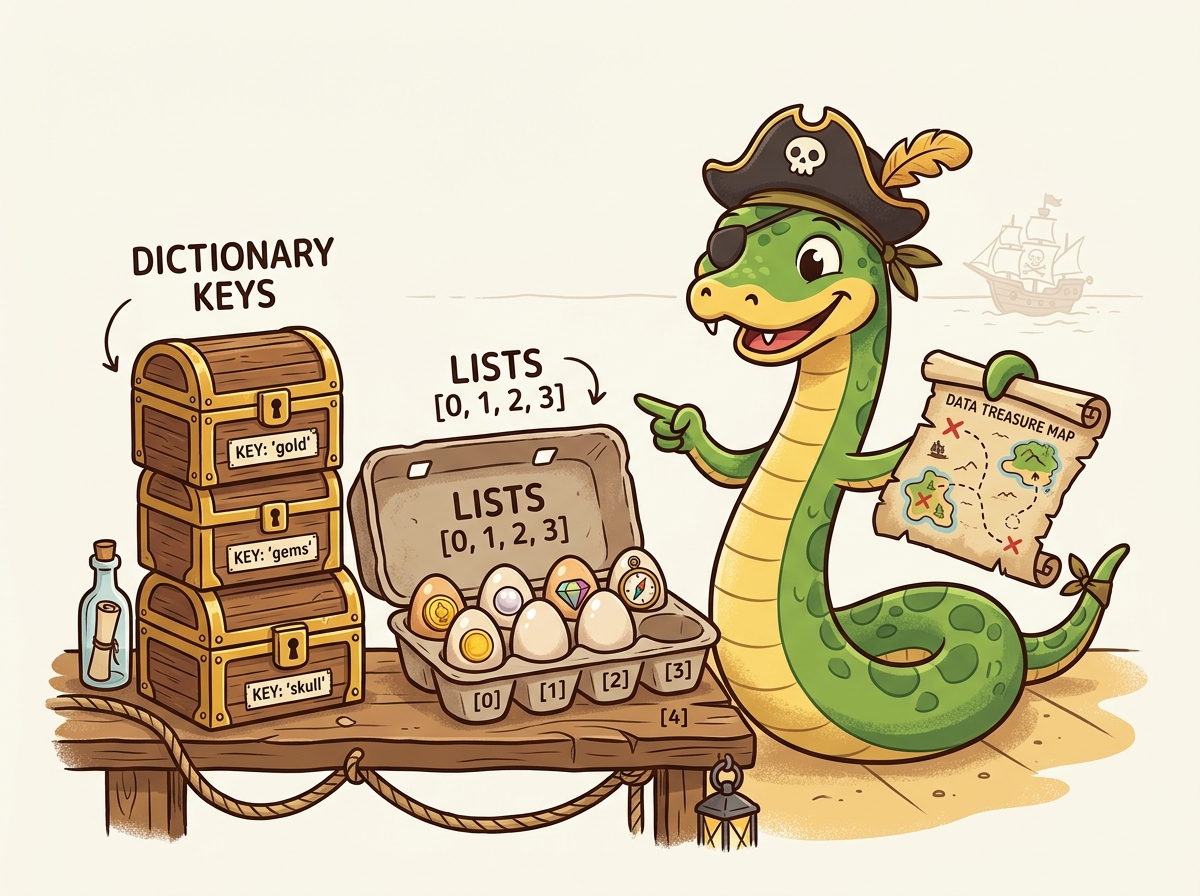
\includegraphics[width=0.75\textwidth]{images/ch5_treasure_chest.jpg}
    \caption{Python data structures organize your data like egg cartons (Lists) and treasure chests (Dictionaries).}
\end{figure}

\section{Beyond Single Variables}

Storing single numbers in individual Tupperware containers is fine for beginners. But what if you have a list of $10,000$ high scores or a map of user profile settings? You need Python's built-in \textbf{data structures}!

\section{Lists: The Infinite Shopping Cart}

A \textbf{list} is an ordered, mutable sequence of items enclosed in square brackets \texttt{[]}.

\begin{pycode}{List Basics}
inventory = ["Magic Wand", "Health Potion", "Shield", "Dragon Tooth"]

# Accessing items (Zero-indexed!)
print("First item:", inventory[0])    # Magic Wand
print("Last item:", inventory[-1])    # Dragon Tooth

# Modifying items
inventory.append("Spellbook")         # Add to end
inventory.remove("Shield")            # Remove by value
print("Updated Inventory:", inventory)
\end{pycode}

\section{Tuples: Carved in Stone}

A \textbf{tuple} is like a list, but it is \textbf{immutable} (unchangeable). Enclosed in round parentheses \texttt{()}.

\begin{pycode}{Tuple Demo}
screen_resolution = (1920, 1080)
# Trying screen_resolution[0] = 3840 will crash with TypeError!
print(f"Width: {screen_resolution[0]}, Height: {screen_resolution[1]}")
\end{pycode}

\section{Dictionaries: Secret Key-Value Maps}

A \textbf{dictionary} stores data in \textbf{key: value} pairs, enclosed in curly braces \texttt{\{\}}. Instead of numeric positions like \texttt{[0]}, you access values by their unique key!

\begin{pycode}{Dictionary Basics}
hero_stats = {
    "name": "Sir Python",
    "level": 42,
    "hp": 250,
    "class": "Snake Wizard"
}

# Accessing and modifying dictionary values
print("Hero Level:", hero_stats["level"])
hero_stats["hp"] += 50   # Drink health potion!
hero_stats["mana"] = 180  # Add new key-value pair

print("Updated Stats:", hero_stats)
\end{pycode}

\section{Sets: Duplicate-Destroying Bouncers}

A \textbf{set} is an unordered collection of unique elements. If you try to add duplicates, a set silently throws them into the trash!

\begin{pycode}{Set Magic}
raw_tags = ["python", "code", "python", "snake", "code", "magic"]
unique_tags = set(raw_tags)
print("Unique Tags:", unique_tags)
\end{pycode}

\section{Code Example: Word Frequency Counter}

Here is how dictionaries and loops collaborate to count how frequently words appear in a sentence.

\begin{pycode}{Word Frequency Counter}
sentence = "python is fun and python is powerful and python is fast"
words = sentence.split()
counts = {}

for word in words:
    if word in counts:
        counts[word] += 1
    else:
        counts[word] = 1

for word, freq in counts.items():
    print(f" - '{word}': {freq} time(s)")
\end{pycode}

\begin{snakesnack}{List Comprehensions: Pythonic Elegance}
Transforming one list into another in a single sleek line of code:
\begin{lstlisting}[language=Python]
numbers = [1, 2, 3, 4, 5]
squares = [x**2 for x in numbers if x % 2 == 0]
print(squares) # Output: [4, 16]
\end{lstlisting}
\end{snakesnack}

\section{Practice Problems \& Exercises}

Unpack your data structures with these 3 practice challenges!

\begin{snakelab}{Problem 5.1: High Score Leaderboard (Easy)}
Given a list of test scores \texttt{scores = [88, 95, 72, 100, 85, 91]}, write code to:
\begin{itemize}
    \item Sort the list in descending order.
    \item Extract the top 3 highest scores using list slicing (\texttt{[:3]}).
    \item Print the average of those top 3 scores!
\end{itemize}
\end{snakelab}

\begin{pycode}{Solution 5.1: High Score Leaderboard}
scores = [88, 95, 72, 100, 85, 91]

scores.sort(reverse=True)
top_3 = scores[:3]
average_top_3 = sum(top_3) / len(top_3)

print("Sorted Leaderboard:", scores)
print("Top 3 Scores:", top_3)
print(f"Top 3 Average: {average_top_3:.1f}")
\end{pycode}

\begin{snakelab}{Problem 5.2: Recipe Ingredient Matcher (Medium)}
Given two sets of ingredients:
\texttt{recipe\_a = \{"flour", "sugar", "eggs", "butter", "vanilla"\}}
\texttt{recipe\_b = \{"flour", "cocoa", "eggs", "butter", "milk"\}}
Write set operations to find:
\begin{enumerate}
    \item Common ingredients in both recipes (intersection \texttt{\&}).
    \item All unique ingredients required across both recipes (union \texttt{\textbar}).
\end{enumerate}
\end{snakelab}

\begin{pycode}{Solution 5.2: Recipe Ingredient Matcher}
recipe_a = {"flour", "sugar", "eggs", "butter", "vanilla"}
recipe_b = {"flour", "cocoa", "eggs", "butter", "milk"}

common = recipe_a & recipe_b
all_unique = recipe_a | recipe_b

print("Common Ingredients:", common)
print("All Required Ingredients:", all_unique)
\end{pycode}

\begin{snakelab}{Problem 5.3: Student Grade Dictionary Lookup (Spicy)}
Create a dictionary mapping student names to lists of grades:
\texttt{grades = \{"Alice": [90, 85, 92], "Bob": [75, 80, 70], "Charlie": [95, 98, 100]\}}
Iterate through the dictionary and print each student's name and their calculated final grade average!
\end{snakelab}

\begin{pycode}{Solution 5.3: Student Grade Lookup}
grades = {
    "Alice": [90, 85, 92],
    "Bob": [75, 80, 70],
    "Charlie": [95, 98, 100]
}

print("--- STUDENT FINAL GRADES ---")
for student, mark_list in grades.items():
    avg = sum(mark_list) / len(mark_list)
    print(f"Student: {student:8s} | Average: {avg:.1f}%")
\end{pycode}

\chapter{Dodging Anvils: Exceptions \& Debugging}

\begin{figure}[h!]
    \centering
    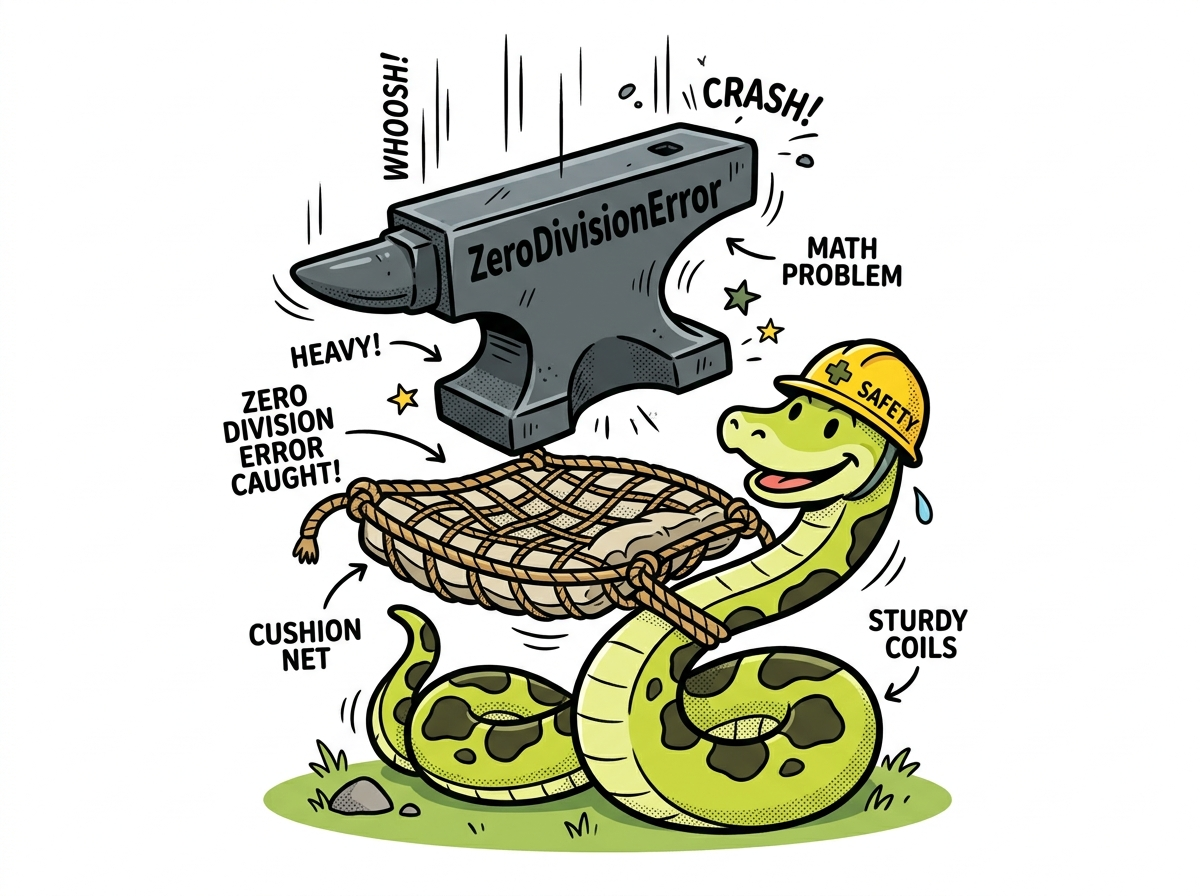
\includegraphics[width=0.75\textwidth]{images/ch6_falling_anvil.jpg}
    \caption{Exception handling is like wearing a hardhat and setting up safety nets to catch falling anvils gracefully.}
\end{figure}

\section{Bugs are Not Monstrous Errors --- They are Clues!}

Every programmer's code breaks. The difference between an amateur and a pro is that an amateur panics when seeing red error text, while a pro puts on detective glasses and reads the traceback!

Python exceptions occur when your code is syntactically valid, but an unexpected event happens at runtime (like dividing by zero or opening a file that doesn't exist).

\section{The Safety Net: \texttt{try} / \texttt{except} Blocks}

Instead of letting your program crash dramatically and scare the user, you can wrap risky code in a \texttt{try} block and catch errors gracefully in an \texttt{except} block.

\begin{pycode}{Catching Division by Zero}
def divide_cookies(total_cookies, people):
    try:
        per_person = total_cookies / people
        print(f"Everyone gets {per_person:.1f} cookies!")
    except ZeroDivisionError:
        print("WHOOPS! You cannot divide cookies among 0 people!")

divide_cookies(10, 2)
divide_cookies(10, 0)
\end{pycode}

\section{Catching Specific Exceptions}

Always catch specific exceptions rather than using a bare \texttt{except:}. Catching specific exceptions prevents you from accidentally swallowing critical system interrupts!

\begin{pycode}{Multiple Exception Handlers}
try:
    user_input = input("Enter a number: ")
    number = int(user_input)
    result = 100 / number
    print("Result:", result)
except ValueError:
    print("Error: That wasn't a valid integer!")
except ZeroDivisionError:
    print("Error: Cannot divide 100 by zero!")
except Exception as e:
    print(f"Unexpected Error: {e}")
\end{pycode}

\section{The Complete Rescue Team: \texttt{else} and \texttt{finally}}

- \textbf{\texttt{else}:} Runs ONLY if NO exceptions occurred in the \texttt{try} block.
- \textbf{\texttt{finally}:} Runs ALWAYS, no matter what happened (great for closing files or cleanup)!

\begin{pycode}{Full Try-Except-Else-Finally Structure}
try:
    print("Opening secret spellbook...")
    file_status = "OPEN"
    # Risky operation
    spell_level = 5
except NameError:
    print("Spell unknown!")
else:
    print("Spell level validated successfully!")
finally:
    file_status = "CLOSED"
    print(f"Cleanup complete. File status: {file_status}")
\end{pycode}

\section{Code Example: Bulletproof User Input Getter}

Here is a practical function pattern used in professional applications to repeatedly prompt users until they provide valid numerical input.

\begin{pycode}{Bulletproof Input Prompt}
def get_positive_integer(prompt_message):
    while True:
        try:
            val = int(input(prompt_message))
            if val <= 0:
                print("Error: Must be greater than 0!")
                continue
            return val
        except ValueError:
            print("Invalid input! Please type a whole number.")

# Simulated usage demo
# age = get_positive_integer("Enter your age: ")
print("Function pattern defined successfully!")
\end{pycode}

\begin{snakesnack}{Reading Stack Traces}
When Python prints a traceback:
1. Look at the **very last line** first! It tells you the exception name (\texttt{KeyError}, \texttt{TypeError}, \texttt{IndexError}).
2. Look at the line number mentioned right above it to pinpoint the exact line of code that triggered the anvil!
\end{snakesnack}

\section{Practice Problems \& Exercises}

Catch falling anvils in these 3 exception exercises!

\begin{snakelab}{Problem 6.1: Safe List Index Access (Easy)}
Write a function \texttt{safe\_get\_item(lst, index)} that returns the item at position \texttt{index}.
If the index is out of bounds, catch the \texttt{IndexError} and return \texttt{"Item Not Found"}.
Test with \texttt{colors = ["Red", "Green", "Blue"]} at index $1$ and index $99$!
\end{snakelab}

\begin{pycode}{Solution 6.1: Safe List Index Access}
def safe_get_item(lst, index):
    try:
        return lst[index]
    except IndexError:
        return "Item Not Found"

colors = ["Red", "Green", "Blue"]
print("Index 1:", safe_get_item(colors, 1))   # Green
print("Index 99:", safe_get_item(colors, 99)) # Item Not Found
\end{pycode}

\begin{snakelab}{Problem 6.2: Safe Dictionary Key Extractor (Medium)}
Write a function \texttt{safe\_dict\_lookup(dictionary, key, default\_value)}:
\begin{itemize}
    \item Try returning \texttt{dictionary[key]}.
    \item If a \texttt{KeyError} occurs, return \texttt{default\_value}.
\end{itemize}
Test looking up \texttt{"mana"} in \texttt{\{"hp": 100, "level": 5\}}.
\end{snakelab}

\begin{pycode}{Solution 6.2: Safe Dictionary Lookup}
def safe_dict_lookup(dictionary, key, default_value):
    try:
        return dictionary[key]
    except KeyError:
        return default_value

player = {"hp": 100, "level": 5}
mana = safe_dict_lookup(player, "mana", 50)
print(f"Player Mana: {mana}") # Returns default 50
\end{pycode}

\begin{snakelab}{Problem 6.3: Custom Range Validation Exception (Spicy)}
Write a function \texttt{set\_volume(level)}:
\begin{itemize}
    \item If \texttt{level} is not an integer, raise a \texttt{TypeError("Volume must be an integer!")}.
    \item If \texttt{level} is outside $0$ to $100$, raise a \texttt{ValueError("Volume must be between 0 and 100!")}.
\end{itemize}
Test calling \texttt{set\_volume(150)} inside a \texttt{try-except} block to catch and print the error message!
\end{snakelab}

\begin{pycode}{Solution 6.3: Custom Range Validation}
def set_volume(level):
    if not isinstance(level, int):
        raise TypeError("Volume must be an integer!")
    if level < 0 or level > 100:
        raise ValueError("Volume must be between 0 and 100!")
    print(f"Volume set to {level}%")

try:
    set_volume(150)
except (TypeError, ValueError) as err:
    print(f"Caught Expected Error: {err}")
\end{pycode}

\chapter{Frankenstein's Workshop: OOP Fundamentals}

\begin{figure}[h!]
    \centering
    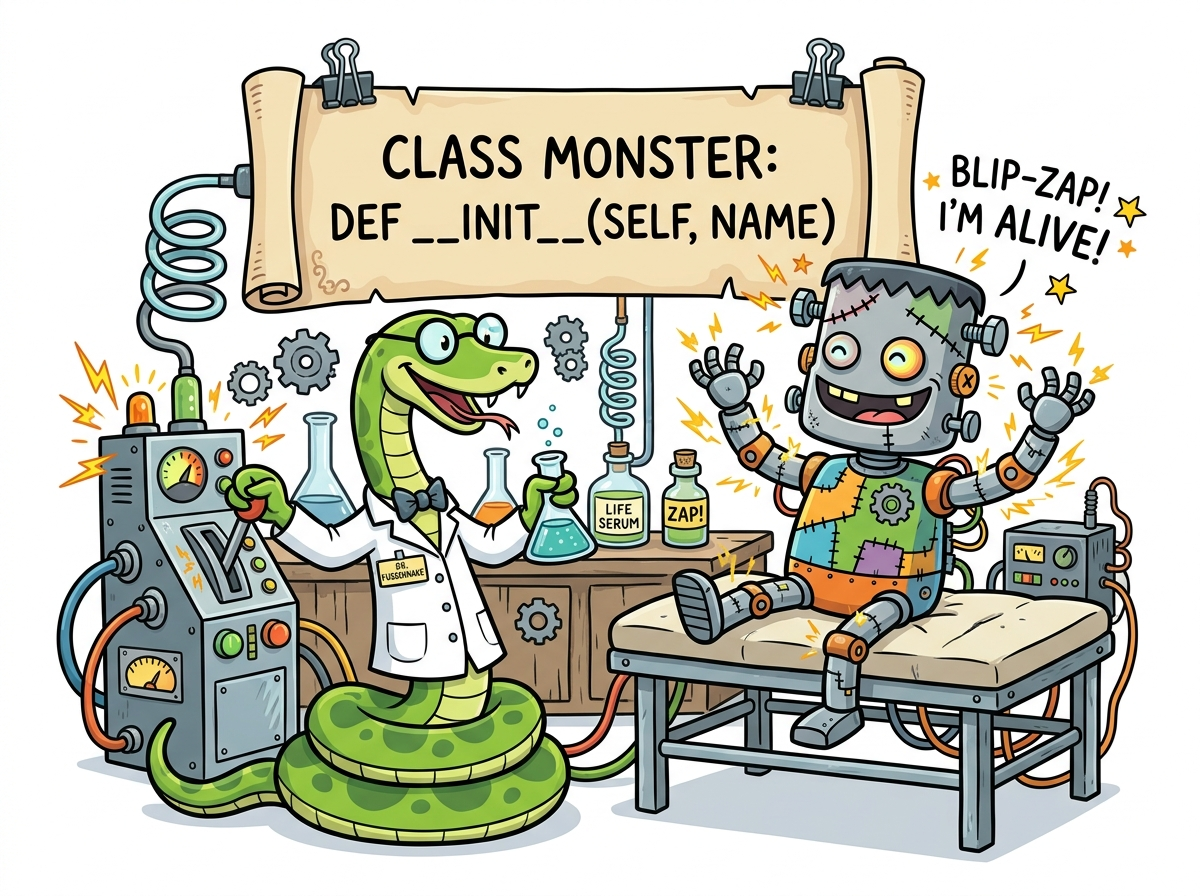
\includegraphics[width=0.75\textwidth]{images/ch7_monster_class.jpg}
    \caption{Classes are architectural blueprints; Objects are the living creations brought to life in memory!}
\end{figure}

\section{Thinking in Objects}

So far, we have treated data and functions as separate entities. But in the real world, things combine both! A car has data (\textit{color}, \textit{speed}) and actions (\textit{accelerate}, \textit{brake}).

\textbf{Object-Oriented Programming (OOP)} is a paradigm where we bundle related data (attributes) and functions (methods) into custom packages called \textbf{Objects}.

\section{Classes vs Objects: The Architectural Blueprint}

- \textbf{Class:} The blueprint or cookie cutter (e.g., \texttt{Monster}).
- \textbf{Object:} An actual instance baked using that cutter (e.g., \texttt{grumpy\_goblin}).

\begin{pycode}{Creating Your First Class}
class Monster:
    # Constructor method: runs when a new object is created
    def __init__(self, name, monster_type, hp):
        self.name = name            # Attribute
        self.monster_type = monster_type  # Attribute
        self.hp = hp                # Attribute

    # Method: Action the object can perform
    def roar(self):
        print(f"ROAR! {self.name} the {self.monster_type} threatens you with {self.hp} HP!")

# Instantiating objects from the class blueprint
goblin = Monster("Griznar", "Goblin", 45)
dragon = Monster("Ignis", "Fire Dragon", 500)

goblin.roar()
dragon.roar()
\end{pycode}

\section{Demystifying \texttt{self}}

Why does every method in a class take \texttt{self} as its first parameter?

Because \texttt{self} refers to the \textbf{specific object} currently calling the method! When \texttt{goblin.roar()} runs, \texttt{self} points to \texttt{goblin}. When \texttt{dragon.roar()} runs, \texttt{self} points to \texttt{dragon}.

\section{Inheritance: Passing Down the Family Genes}

You don't need to write every class from scratch! A child class can \textbf{inherit} attributes and methods from a parent class, and then add its own unique powers.

\begin{pycode}{Class Inheritance}
# Base Parent Class
class Hero:
    def __init__(self, name):
        self.name = name
        self.health = 100

    def rest(self):
        self.health += 20
        print(f"{self.name} rested. Health is now {self.health}.")

# Child Class inheriting from Hero
class Wizard(Hero):
    def __init__(self, name, mana):
        super().__init__(name) # Call Parent Constructor
        self.mana = mana

    def cast_spell(self):
        self.mana -= 10
        print(f"{self.name} cast a spell! Mana remaining: {self.mana}")

# Using the Wizard
merlin = Wizard("Merlin the Great", 100)
merlin.cast_spell()
merlin.rest() # Inherited from Hero parent class!
\end{pycode}

\section{Code Example: Bank Account Class with Encapsulation}

Here is a practical financial account class demonstrating data validation inside methods.

\begin{pycode}{BankAccount Class}
class BankAccount:
    def __init__(self, owner, initial_balance=0.0):
        self.owner = owner
        self.balance = initial_balance

    def deposit(self, amount):
        if amount > 0:
            self.balance += amount
            print(f"Deposited ${amount:.2f}. New Balance: ${self.balance:.2f}")

    def withdraw(self, amount):
        if 0 < amount <= self.balance:
            self.balance -= amount
            print(f"Withdrew ${amount:.2f}. Remaining Balance: ${self.balance:.2f}")
        else:
            print("Insufficient funds or invalid withdrawal amount!")

account = BankAccount("Alice", 100.00)
account.deposit(50.00)
account.withdraw(30.00)
\end{pycode}

\begin{snakesnack}{OOP Golden Rules}
1. Keep class names in \texttt{CamelCase} (e.g. \texttt{SpaceShip}, \texttt{UserProfile}).
2. Use attributes for *nouns* (data) and methods for *verbs* (actions).
3. Inheritance promotes code reuse, but don't over-engineer giant complex family trees!
\end{snakesnack}

\section{Practice Problems \& Exercises}

Bring your blueprints to life with these 3 OOP practice problems!

\begin{snakelab}{Problem 7.1: Car Mileage Tracker (Easy)}
Create a \texttt{Car} class with attributes \texttt{make}, \texttt{model}, and \texttt{odometer} (default $0$).
Add a method \texttt{drive(miles)} that increases \texttt{odometer} by \texttt{miles}.
Instantiate a car object, drive it twice, and print its odometer reading!
\end{snakelab}

\begin{pycode}{Solution 7.1: Car Mileage Tracker}
class Car:
    def __init__(self, make, model):
        self.make = make
        self.model = model
        self.odometer = 0

    def drive(self, miles):
        self.odometer += miles
        print(f"Drove {miles} miles. Odometer: {self.odometer} miles.")

my_car = Car("Cyber", "Truck")
my_car.drive(120)
my_car.drive(85)
\end{pycode}

\begin{snakelab}{Problem 7.2: Digital Shopping Cart (Medium)}
Create a \texttt{ShoppingCart} class:
\begin{itemize}
    \item Attribute: \texttt{items} (dictionary of item\_name -> price).
    \item Methods: \texttt{add\_item(name, price)}, \texttt{get\_total()}.
\end{itemize}
Instantiate a cart, add 3 items, and print the calculated total cost!
\end{snakelab}

\begin{pycode}{Solution 7.2: Digital Shopping Cart}
class ShoppingCart:
    def __init__(self):
        self.items = {}

    def add_item(self, name, price):
        self.items[name] = price

    def get_total(self):
        return sum(self.items.values())

cart = ShoppingCart()
cart.add_item("Python Book", 29.99)
cart.add_item("Coffee Mug", 12.50)
cart.add_item("Keyboard", 89.00)

print(f"Total Cart Value: ${cart.get_total():.2f}")
\end{pycode}

\begin{snakelab}{Problem 7.3: Employee \& Manager Hierarchy (Spicy)}
Create an \texttt{Employee} class with \texttt{name} and \texttt{salary}.
Create a child class \texttt{Manager(Employee)} with an additional attribute \texttt{department} and a method \texttt{hire\_bonus()} that increases their salary by \$5,000!
\end{snakelab}

\begin{pycode}{Solution 7.3: Employee Hierarchy}
class Employee:
    def __init__(self, name, salary):
        self.name = name
        self.salary = salary

class Manager(Employee):
    def __init__(self, name, salary, department):
        super().__init__(name, salary)
        self.department = department

    def hire_bonus(self):
        self.salary += 5000
        print(f"Manager {self.name} ({self.department}) received bonus! Salary: ${self.salary}")

boss = Manager("Sarah", 85000, "Engineering")
boss.hire_bonus()
\end{pycode}


% --- Back Matter: Cheat Sheet & Conclusion ---
\backmatter
\chapter{The Ultimate Python Cheat Sheet}

\begin{snakesnack}{Quick Reference Guide}
Here is your emergency rescue pocket guide to Python syntax!
\end{snakesnack}

\begin{pycode}{Python Syntax Cheat Sheet}
# 1. Variables & Types
age = 20                 # int
pi = 3.14159             # float
name = "Snake"           # str
is_wizard = True         # bool

# 2. String Formatting
greeting = f"Hello {name}, you are level {age}!"

# 3. Control Flow
if age >= 18:
    print("Adult")
elif age >= 13:
    print("Teen")
else:
    print("Child")

# 4. Loops
for i in range(3):        # 0, 1, 2
    print(i)

while is_wizard:
    print("Casting spells!")
    break                 # Exit loop

# 5. Functions
def add(a, b=5):
    return a + b

# 6. Data Structures
my_list = [1, 2, 3]       # Ordered, mutable
my_tuple = (10, 20)       # Immutable
my_dict = {"a": 1, "b": 2}# Key-Value map
my_set = {1, 2, 3}        # Unique elements

# 7. Error Handling
try:
    val = 10 / 0
except ZeroDivisionError:
    print("Caught division by zero!")

# 8. OOP Class
class Snake:
    def __init__(self, name):
        self.name = name
    def hiss(self):
        print(f"{self.name} says HISS!")
\end{pycode}

\vspace{1cm}
\begin{center}
{\Large \bfseries \color{pypurple} Congratulations! You are now a Certified Python Wizard!} \\
\vspace{0.3cm}
{\color{codegray} Keep experimenting, build fun projects, and never fear a traceback!}
\end{center}

\end{document}
